%!TEX root = ../phd-thesis-lei-ma.tex

%%%%%%%%%%%%%%%%%%%%%%%%%%%%%%%%%%%%%%%%%%
%%%%%%%%%%%%% APPENDIX  %%%%%%%%%%%%%%%%%%
%%%%%%%%%%%%%%%%%%%%%%%%%%%%%%%%%%%%%%%%%%


\part*{Appendices}
\label{chap:appendices}
\addcontentsline{toc}{chapter}{Appendices}
 % Next lines duplicated from .toc file and used to create mini
 % "Appendix Table of Contents," if desired:
   % \contentsline {chapter}{\numberline {A} Notations}{}
   % \contentsline {chapter}{\numberline {B} Conventions}{}
   % \contentsline {chapter}{\numberline {C} Rabi Oscillations}{}
   % \contentsline {chapter}{\numberline {D} MSW Effect Revisited}{}
%   \contentsline {chapter}{\numberline {B}Derivation of $A = \pi r^2$}{5}
 % End mini table of contents

\appendix



\chapter{\label{chap:app-sec:conventions}Conventions}

\section{\label{part:app-chap:conventions-sec:notations}Notations}

\begin{itemize}
  \item Variables with sans-serif fonts are matrices.
  \item Variables in bold are vectors in space-time.
  \item Variables with arrows are vectors in flavor-isospin space.
\end{itemize}

\section{\label{chap:app-sec:conventions-subsec:terms}Terms}

\begin{itemize}
    \item
    Normal hierarchy for two-flavor scenario is always defined as $m_2^2-m_1^2>0$, i.e., $\omega_{\mathrm v}>0$.
    \item
    Inverted hierarchy for two-flavor scenario is defined as $m_2^2-m_1^2<0$, i.e., $\omega_{\mathrm v}<0$.
    \item
    Solar neutrino mass splitting is $\delta m_{12}$, while atmospheric neutrino mass splitting refers to $\delta m_{23}$.
\end{itemize}





\section{\label{chap:app-sec:conventions-subsec:units}Units}


Natural units system makes the calculations of neutrinos convenient. By definition, we set reduced Planck constant and speed of light to be 1, $\hbar = 1 = c$.
The conversion between natural units and SI can be down by using the following relations,
\begin{align}
   1 \mathrm{GeV} &= 5.08 \times 10^{15} \mathrm {m^{-1}} \\
   1 \mathrm{GeV} &= 1.8\times 10^{-27} \mathrm{kg}
\end{align}
To convert between different physical quantities in this thesis, I always use the following tips.
\begin{itemize}
    \item The energy-mass-momentum relations becomes $E^2 = p^2 + m^2c^2 = p^2 + m^2$. Thus mass $m$, momentum $\mathbf p$ and energy $E$ have the same dimension.
    \item An example of angular momentum in quantum mechanics is $L_z = m\hbar = m$ where $m$ is a quantum number. $\hbar$ is of dimension angular momentum.
    \item A plane wave in quantum mechanics is $\Psi = A e^{ \frac{E t - p x}{\hbar} }$. $\frac{E t - p x}{\hbar}$ should be dimensionless, which means $px$ has dimension angular momentum, which is obvious, meanwhile we notice that $E t$ also has the dimension of angular momentum. Previously we noticed momentum has the same dimension with energy, we should have time $t$ with the same dimension of length $x$. Also we can conclude that length and time have the same dimension as $1/E$.
\end{itemize}



\section{Pauli Matrices and Rotations}


Given a rotation
\begin{equation}
   U = \begin{pmatrix} \cos \theta & \sin \theta \\ -\sin\theta & \cos \theta \end{pmatrix},
\end{equation}
its effect on Pauli matrices are
\begin{align}
      U^\dagger \sigma_3 U  &=\cos 2\theta \sigma_3 + \sin 2\theta \sigma_1 \\
  U^\dagger \sigma_1 U & = -\sin 2\theta \sigma_3 + \cos 2\theta \sigma_1.
\end{align}


\section{Lorentzian Distribution}


Three-parameter Lorentzian function is
\begin{equation}
  f_{x_0,\sigma,A}(x)= \frac{1}{\pi} \frac{\sigma}{\sigma^2 + (x-x_0)^2},
\end{equation}
which has a width $2\gamma$.


\section{Fourier Series}

The convention for the Fourier series used in this thesis is
\begin{equation}
\lambda(x) = \sum_{n=-\infty}^{\infty} \Lambda_n \exp\left( \frac{i2\pi n x}{X} \right) = \sum_{n=-\infty}^{\infty} \Lambda_n \exp\left( i \omega_0 n x \right),
\end{equation}
where $\omega_0 = \frac{2\pi}{X}$. The coefficients are evaluated using the orthogonal relation of exponential functions for $n\neq 0$,
\begin{align}
   \Lambda_n &= \frac{1}{X} \int_0^X \lambda(x) e^{ - i \omega_0 n x} dx \\
   & = \frac{1}{X} \left( \int_{0}^{X_1} \lambda_1 e^{ - i \omega_0 n x} dx + \int_{X_1}^{X_1+X_2} \lambda_2 e^{ - i \omega_0 n x} dx  \right) \\
   & = \frac{1}{X} \frac{X}{-i2\pi n} \left( \lambda_1 e^{-i\omega_0 n X_1} + \lambda_2 \left( e^{-i\omega_0 n X} - e^{-i\omega_0 n X_1}  \right) \right) \\
   & = \frac{i}{2\pi n} \left( -\lambda_1 + (\lambda_1 - \lambda_2) e^{-i2\pi n X_1/X} + \lambda_2 e^{-i 2\pi n} \right).
   \label{app-chap:convention-sec:fourier-series-eqn:parametric-resonance-castle-wall-fourier-coeff}
\end{align}
For $n=0$, we have
\begin{equation}
   \Lambda_0 = \frac{X_1 \lambda_1 + X_2 \lambda_2}{X}.
\end{equation}




For functions with specific parity, the Fourier series is much more simpler. I'll list below the Fourier series for even functions, since no odd functions are used in this thesis. In general the Fourier series of a periodic function defined on $\left[ -\frac{X}{2}, \frac{X}{2} \right]$ is
\begin{equation}
      \lambda(x) = \frac{a_0}{2} + \sum_{n=1}^\infty a_n \cos(n 2\pi x/X) + \sum_{n=1}^\infty b_n \sin(n 2\pi x/X),
\end{equation}
where
\begin{align}
    a_0 & = \frac{2}{X} \int^{X/2}_{-X/2} \lambda(x) d x \\
    a_n & = \frac{2}{X} \int_{-X/2}^{X/2} \lambda(x) \cos ( n2\pi x/X ) dx\\
    b_n & = \frac{2}{X} \int_{-X/2}^{X/2} \lambda(x) \sin( n 2\pi x/X ) dx.
\end{align}
For even function $\lambda(x)$, we have
\begin{equation}
      \lambda(x) = \frac{1}{2}a_0 + \sum_{n=1}^\infty a_n \cos (n 2\pi x/X).
\end{equation}

\begin{figure}
    \centering
    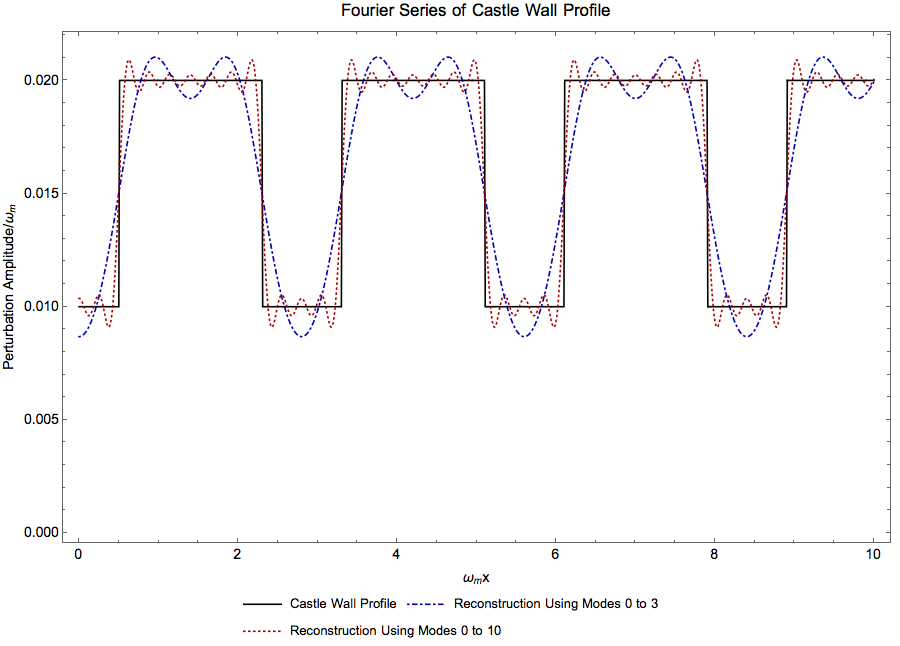
\includegraphics[width=\textwidth]{chapters/assets/app/reconstruction-of-even-castle-wall-0point01-0point02-1-1point8.png}
    \caption{Approaching an even function with Fourier series. The blue dash dotted line is the reconstruction of castle wall profile using 0 to 3 Fourier modes. The red dotted line is the reconstruction using 0 to 10 Fourier modes. }
    \label{app-chap:convention-sec:fourier-series-eqn:parametric-resonance-castle-wall-fourier-coeff-even}
\end{figure}

We shift the castle wall profile and make it always even, as shown in Fig.~\ref{app-chap:convention-sec:fourier-series-eqn:parametric-resonance-castle-wall-fourier-coeff-even}, so that
\begin{equation}
   \lambda(x) = \begin{cases} \lambda_2 , &\quad -\frac{X_2}{2}-\frac{X_1}{2}\le x\le -\frac{X_1}{2} \\
   \lambda_1, &\quad -\frac{X_1}{2}\le x\le \frac{X_1}{2} \\
   \lambda_2, &\quad \frac{X_1}{2}\le x\le \frac{X_1}{2}+\frac{X_2}{2}
   \end{cases}
\end{equation}
Fourier series of the profile is
\begin{equation}
   \lambda(x) = \frac{1}{2}\Lambda_0 + \sum_{q=1}^{\infty} \Lambda_q \cos\left( \frac{ 2\pi q x}{X} \right) = \frac{1}{2} \Lambda_0 + \sum_{q=1}^{\infty} \Lambda_q \cos\left( \omega_0 q x \right),
\end{equation}
where
\begin{align}
   \Lambda_0 =& \frac{2}{X} \int^{X/2}_{-X/2} \lambda(x) d x \\
    =& \frac{2}{X} \left(  \lambda_2 X_2 + \lambda_1 X_1   \right) \\
   \Lambda_q &= \frac{2}{X} \int_{-X/2}^{X/2} \lambda(x) \cos(n 2\pi x/X)dx \\
    =& \frac{2}{X} \left( \lambda_2 \int_{-X/2}^{-X_1/2} \cos(n 2\pi x/X)dx + \lambda_1 \int_{-X_1/2}^{X_1/2} \cos(n 2\pi x/X)dx \right. \\
   &\left.+ \lambda_2 \int_{X_1/2}^{X/2} \cos(n 2\pi x/X)dx \right) \\
    =& \frac{2}{q\pi} \left( \lambda_2\left( \sin(q\omega_0 X/2) - \sin(q\omega_0 X_1/2) \right) + \lambda_1 \sin( q\omega_0 X_1/2)  \right)  \\
    =& \frac{2}{q\pi} \left( \lambda_2\left( \sin(q \pi ) - \sin(q \pi X_1/X) \right) + \lambda_1 \sin( q\pi X_1/X)  \right)
\end{align}


\section{Jacobi-Anger expansion}

One of the forms of Jacobi-Anger expansion is
\begin{equation}
    e^{i z \cos (\Phi)} = \sum_{n=-\infty}^\infty i^n J_n(z) e^{i n\Phi}.
    \label{eqn:jacobi-anger-expansion}
\end{equation}


\section{Bessel Functions}

A special relation of Bessel function is that
\begin{equation}
  J_n(n \sech \alpha) \sim \frac{ e^{n(\tanh\alpha - \alpha)} }{\sqrt{ 2\pi n \tanh \alpha } }
\end{equation}
for large $n$~\cite{Ploumistakis2009}. As a matter of fact, for all positive $\alpha$, we always have $\tanh \alpha - \alpha < 0$.

Using this relation and defining $\sech \alpha = A \cos 2\theta_m$, which renders
\begin{equation}
  \alpha = 2 n \pi i + \ln \left(  \frac{ 1 \pm \sqrt{ -A^2 \cos^2 2\theta_m + 1 } }{ A\cos 2\theta_m } \right),\qquad n\in \mathrm{Integers},
  \label{eqn-width-alpha-solved}
\end{equation}
where the Mathematica code to solve it is shown below,
\begin{verbatim}
In[1]:= Solve[Exp[z] + Exp[-z]
== 2/(A Cos[2 Subscript[\[Theta], m]]), z] // FullSimplify
\end{verbatim}
we find out an more human readable analytical expression for the width
\begin{equation}
  \Gamma = \left\lvert 2 \hat k \tan 2\theta_m \frac{ e^{n ( \tanh \alpha - \alpha )} }{n_0 \sqrt{2\pi n_0 \tanh \alpha} } \right\rvert
\end{equation}
where $\alpha$ is solved out in \ref{eqn-width-alpha-solved}.
For small $\alpha$, we have expansions for exponential functions and hyperbolic functions $\tanh \alpha \sim \alpha - \frac{\alpha^3}{3}$,
\begin{equation}
  \Gamma \asymp 2\tan 2\theta_m \frac{ e^{n \alpha^3/3} }{\sqrt{2\pi \alpha} n_0^{3/2}  }.
\end{equation}
However, it doesn't really help that much since $n$ is large and no expansion could be done except for significantly small $\alpha$.





\section{Conversions in Neutrino Physics}

Using natural units, length = time = 1/energy, we could rescale almost all quantities in neutrino oscillations using energy, or whatever characteristic scale we have.

We use two flavor vacuum oscillations between the two masses $m_1$ and $m_2$ as an example. The characteristic energy scale is the oscillation frequency $\omega_{v,21}$. The equation of motion
\begin{align}
   i\frac{d}{d x} \Psi = \frac{\omega_v}{2}(-\cos 2\theta_v \boldsymbol{\sigma_3} + \sin 2\theta_v \boldsymbol{\sigma_1}) \Psi,
\end{align}
can be rescaled using the characteristic energy scale $\omega_{v,21}$
\begin{align}
   i\frac{d}{d \hat x} \Psi = \frac{1}{2}(-\cos 2\theta_v \boldsymbol{\sigma_3} + \sin 2\theta_v \boldsymbol{\sigma_1})\Psi ,
\end{align}
where $\hat x = \omega_{v,21} x$. It is convenient for numerical calculations to convert quantities into dimensionless ones.

However, we usually discuss oscillation length in SI units for a grip of the picture. To convert from natural units to SI units, we write down the conversion here. The oscillation angular frequency is given by
\begin{align}
   \omega_{v,21} &= \frac{\delta m^2}{2E} \nonumber\\
   &=  \left(\frac{7.5\times 10^{-5}\mathrm{eV}^2}{2\times 1\mathrm{MeV}} \right) \left(\frac{\delta m^2}{7.5\times 10^{-5}\mathrm{eV}^2} \right) \frac{1\mathrm{MeV}}{E} \nonumber\\
   &= 3.75\times 10^{-11}\mathrm{eV}  \left(\frac{\delta m^2}{7.5\times 10^{-5}\mathrm{eV}^2}\right) \left(\frac{1\mathrm{MeV}}{E}\right) .
\end{align}
On the other hand, electro-volt is related to length through the useful formula
\begin{equation}
   197\mathrm{MeV}\cdot \mathrm{fm} = \hbar c = 1.
\end{equation}
Thus we have the oscillation angular frequency written as
\begin{align}
   \omega_{v,21} &= 3.75\times 10^{-11}\mathrm{eV}  \frac{\delta m^2}{7.5\times 10^{-5}\mathrm{eV}^2} \frac{1\mathrm{MeV}}{E} \nonumber\\
   &= 3.75\times 10^{-17}\mathrm{MeV}  \frac{\delta m^2}{7.5\times 10^{-5}\mathrm{eV}^2} \frac{1\mathrm{MeV}}{E}\nonumber \\
   &= 1.90\times 10^{-4}  \mathrm{m}^{-1}  \frac{\delta m^2}{7.5\times 10^{-5}\mathrm{eV}^2} \frac{1\mathrm{MeV}}{E}.
   \label{common-sense-eqn-omega-v-si-unit}
\end{align}
Similarly for $\delta m_{32}=2.4\times 10^{-3}\mathrm{eV^2}$ the frequency is
\begin{align}
   \omega_{v,32} =\frac{\delta m^2_{32}}{2E} = 6.3\times 10^{-3} \mathrm{m}^{-1}  \frac{\delta m^2_{32}}{2.5\times 10^{-3} \mathrm{eV}^2 } \frac{1MeV}{E}.
\end{align}
With the results for angular frequencies, the rescaled length $\hat x$ is restored using
\begin{align}
    x = \frac{\hat x}{\omega_v} &= \frac{\hat x}{  1.90\times 10^{-4}  \mathrm{m}^{-1}  \frac{\delta m^2}{7.5\times 10^{-5}\mathrm{eV}^2} \frac{1\mathrm{MeV}}{E} } \\
    &= \frac{\hat x}{0.190} \mathrm{km} \frac{7.5\times 10^{-5}\mathrm{eV}^2}{\delta m^2}  \frac{E}{1\mathrm{MeV}}.
\end{align}


Another important example is the 2 flavor neutrino oscillations in constant matter background potential $\lambda_c = \sqrt{2}G_{\mathrm F} n_e$. The characteristic energy scale is $\omega_m$ which is calculated using
\begin{equation}
   \omega_m = \omega_v \sqrt{ \frac{\lambda_c}{\omega_v}^2 + 1 - 2 \frac{\lambda_c}{\omega_v}\cos 2\theta_v }.
   \label{common-sense-eqn-omega-m}
\end{equation}
Meanwhile, the effective mixing angle $\theta_m$ is determined by
\begin{equation}
   \tan 2\theta_m = \frac{\sin 2\theta_v}{\cos 2\theta_v - \frac{\lambda}{\omega_v} }.
\end{equation}
Similar to vacuum equation of motion, we rescale the equation of motion in constant background using $\omega_m$
\begin{equation}
   i \frac{d}{d\hat x} \Psi = \frac{1}{2}(-\cos 2\theta_m \boldsymbol{\sigma_3} + \sin 2\theta_m \boldsymbol{\sigma_1})\Psi ,
\end{equation}
we find out the scaled distance
\begin{equation}
   \hat x = \omega_m x.
\end{equation}
To reverse the process and find out the actual SI unit distance after the numerical calculation, we use
\begin{equation}
   x = \frac{\hat x}{\omega_m}.
   \label{common-sense-eqn-actual-distance-constant-matter}
\end{equation}
The procedure will be the following.
\begin{itemize}
    \item Calculate $\omega_v$ using Eq.~\ref{common-sense-eqn-omega-v-si-unit}.
\item Calculate $\hat\lambda_c = \frac{\lambda_c}{\omega_v}$.
\item Calculate $\omega_m$ using Eq.~\ref{common-sense-eqn-omega-m}.
\item Find out the actual distance using Eq.~ \ref{common-sense-eqn-actual-distance-constant-matter}.
\end{itemize}





%%%%%%%%%%%%%%%%%%%%%%%%%%%%%%%%%%%%%%%%%%%%%%%%%%%%%%%%%
%%%%%%%%%%%% MSW Revisted %%%%%%%%%%%%%%%%%%%%%%%%%%%%%%%%%%


\chapter{\label{app:msw-revisited}MSW Effect Revisited}






\section{Flavor Basis}

In terms of formalism, vacuum oscillations is already a Rabi oscillation at resonance with oscillation width $\omega_v \sin 2\theta_v$. As derived, neutrino oscillations in matter are determined by Hamiltonian in flavor basis
\begin{equation}
      H^{(f)} = \left(- \frac{1}{2} \omega_v \cos 2\theta_v +\frac{1}{2}\lambda(x)  \right)\sigma_3 + \frac{1}{2} \omega_v \sin 2\theta_v \sigma_1,
\end{equation}
with the Schr\"{o}ding equation
\begin{equation}
    i \partial_x \Psi^{(f)} = H^{(f)} \Psi^{(f)}.
\end{equation}
To make connections to Rabi oscillations, we would like to remove the changing $\sigma_3$ terms, using a transformation
\begin{equation}
    U = \begin{pmatrix} e^{-i \eta (x)} & 0 \\  0 & e^{i \eta (x)}  \end{pmatrix},
\end{equation}
which transform the flavor basis to another basis
\begin{equation}
    \begin{pmatrix} \psi_e \\ \psi_x \end{pmatrix} = \begin{pmatrix} e^{-i \eta (x)} & 0 \\  0 & e^{i \eta (x)}  \end{pmatrix} \begin{pmatrix} \psi_{a} \\ \psi_{b} \end{pmatrix}.
\end{equation}
The Schrodinger equation can be written into this new basis
\begin{equation}
    i \partial_x (T \Psi^{(r)}) = H^{(f)} T\Psi^{(r)},
\end{equation}
which is simplified to
\begin{equation}
    i \partial_x \Psi^{(r)} = H^{(r)} \Psi^{(r)},
\end{equation}
where
\begin{equation}
 H^{(r)} = - \frac{1}{2}\omega_v \cos 2\theta_v \sigma_3 + \frac{1}{2} \omega_v \sin 2\theta_v \begin{pmatrix}
   0 & e^{2i\eta(x)} \\
   e^{-2i\eta(x)} & 0 \\
   \end{pmatrix},
\end{equation}
in which we remove the varying component of $\sigma_3$ elements using
\begin{equation}
    \frac{d}{dx}\eta(x) = \frac{\lambda(x)}{2}.
\end{equation}
The final Hamiltonian would have some form
\begin{equation}
     H^{(r)} = - \frac{1}{2}\omega_v \cos 2\theta_v \sigma_3 + \frac{1}{2} \omega_v \sin 2\theta_v \begin{pmatrix}
   0 & e^{i\int_0^x \lambda(\tau)d\tau + 2i\eta(0)} \\
   e^{-i\int_0^x \lambda(\tau)d\tau - 2i\eta(0)} & 0 \\
   \end{pmatrix},
\end{equation}
where $\eta(0)$ is chosen to counter the constant terms from the integral.

For arbitrary matter profile, we could first apply Fourier expand the profile into trig function then use Jacobi-Anger expansion so that the system becomes a lot of Rabi oscillations.
Any transformations or expansions that decompose $\exp{\left(i\int_0^x \lambda(\tau)d\tau\right)}$ into many summations of $\exp{\left( i a x + b \right)}$ would be enough for an Rabi oscillation interpretation.
As for constant matter profile, $\lambda(x) = \lambda_0$, we have
\begin{equation}
     \eta(x) = \frac{1}{2} \lambda_0 x.
\end{equation}
The Hamiltonian becomes
\begin{equation}
     H^{(r)} = - \frac{1}{2}\omega_v \cos 2\theta_v \sigma_3 + \frac{1}{2} \omega_v \sin 2\theta_v \begin{pmatrix}
   0 & e^{i\lambda_0 x} \\
   e^{-i\lambda_0 x} & 0 \\
   \end{pmatrix},
\end{equation}
which is exactly a Rabi oscillation. The resonance condition is
\begin{equation}
   \lambda_0 = \omega_v \cos 2\theta_v.
\end{equation}





\section{Instantaneous Matter Basis}


Neutrino oscillations can be calculated in instantaneous matter basis, where the Schr\"{o}dinger equation is transformed to instantaneous matter basis by applying a rotation $U$,
\begin{equation}
    i \partial_x \left(  U\Psi^{(m)} \right)= H^{(f)} U\Psi^{(m)},
\end{equation}
where
\begin{equation}
    U = \begin{pmatrix} \cos \theta_m & \sin \theta_m \\ -\sin\theta_m & \cos \theta_m \end{pmatrix}.
\end{equation}
With some simple algebra, we can write the system into
\begin{equation}
    i \partial _x \Psi^{(m)} = H^{(m)}\Psi^{(m)} ,
\end{equation}
where
\begin{equation}
    H^{(m)} = U^\dagger H^{(f)} U - i U^\dagger \partial_x U.
\end{equation}
By setting the off-diagonal elements of the first term $U^\dagger H^{(f)} U$ to zero, we can derive the relation
\begin{equation}
   \tan 2\theta_m = \frac{\sin 2\theta_v}{\cos 2\theta_v - \lambda/\omega_v}.
\end{equation}
Furthermore, we derive the term
\begin{equation}
    i U^\dagger \partial_x U = - \dot\theta_m \sigma_2.
\end{equation}
We can calculate $\dot\theta_m$ by taking the derivative of $\tan 2\theta_m$,
\begin{equation}
    \frac{d}{dx} \tan 2\theta_m = \frac{2}{\cos^2 2\theta_m} \dot\theta_m,
\end{equation}
so that
\begin{align}
    \dot\theta_m &= \frac{1}{2} \cos^2 (2\theta_m) \frac{d}{dx} \tan 2\theta_m \\
   & = \frac{1}{2} \frac{(\cos 2\theta_v - \lambda/\omega_v)^2}{ (\lambda/\omega_v)^2 + 1 - 2\lambda \cos 2\theta_v /\omega_v } \frac{d}{dx} \frac{\sin 2\theta_v}{\cos 2\theta_v - \lambda/\omega_v} \\
   & = \frac{1}{2} \frac{(\cos 2\theta_v - \lambda/\omega_v)^2}{ (\lambda/\omega_v)^2 + 1 - 2\lambda \cos 2\theta_v /\omega_v }  \frac{\sin 2\theta_v}{(\cos 2\theta_v - \lambda/\omega_v)^2} \frac{1}{\omega)v} \frac{d}{dx} \lambda(x) \\
   & = \frac{1}{2} \sin 2\theta_m \frac{1}{\omega_m} \frac{d}{dx} \lambda(x).
\end{align}



%%%%%%%%%% MSW Revisted %%%%%%%%%%%%%%%%%%%%%%%%%%%%%
%%%%%%%%%%%%%%%%%%%%%%%%%%%%%%%%%%%%%%%%%%%%%%%%%%%%%




%%%%%%%%%%%%%%%%%%%%%%%%%%%%%%%%%%%%%%%%%%%%%%%%%%%%%
%%%%%%%%%% Bipolar %%%%%%%%%%%%%%%%%%%%%%%%%%%%%

\section{\label{chap:app-sec:bipolar}Bipolar Model}

The nature of this section is to provide the linear stability analysis of bipolar model. Bipolar model is a model of neutrino oscillations with the presence of neutrino and antineutrinos. It is also called bimodal oscillations~\cite{Samuel1996}, which means two frequencies in the context. An example of such instability happens in a system composed of equal amounts of neutrinos and antineutrinos.

% Vacuum mixing angle triggers the flavour instability.

Neutrino oscillations has a small amplitude inside a SN core (suppressed by matter effects)~\cite{wolf78}, which basically pins down the flavour transformation. As the neutrinos reaches a further distance, matter effect could drop out. Neutrino self-interaction becomes more important. S. Samuel considers a system of neutrinos and antineutrinos with only vacuum and neutrino self-interactions~\cite{Samuel1996}. The neutrinos and antineutrino forms a bipolar vector in flavor isospin space. The flavor isospin of neutrinos and that of antineutrinos are coupled.

% H. Duan decomposed the system into "normal modes" of the flavor isospin. The bipolar system is discussed in details in this paper. In a two beam model, the length of one of the perturbations can be described using an equation

% .. math::
%   \ddot {\tilde q_+} \approx - \eta (\eta + \mu) \tilde q_+,

% where :math:`\eta=\pm 1` deterimines the hierarchy, :math:`\mu=2\sqrt{2}G_F \lvert \omega_0 \rvert^{-1} n_{\mathrm {tot}}`. We find out from the equation that normal hierarchy (NH, :math:`\eta=1`) doesn't have instabilities, but inverted hierarchy (IH, :math:`\eta=-1`) has instabilities with growth rate :math:`\sqrt{\mu-1}`, if :math:`\mu>1`.



The equation of motion is
\begin{align*}
   i\partial_t \rho =& \left[ -\frac{\omega_v}{2} \cos2\theta \sigma_3 + \frac{\omega_v}{2}\sin 2\theta \sigma_1 - \mu \alpha \bar \rho , \rho\right] \\
   i\partial_t \bar\rho =& \left[ \frac{\omega_v}{2} \cos2\theta \sigma_3 - \frac{\omega_v}{2}\sin 2\theta \sigma_1 + \mu \rho , \bar\rho\right].
\end{align*}
For the purpose of linear stability analysis, we assume that
\begin{align*}
   \rho =& \frac{1}{2}\begin{pmatrix}
   1 & \epsilon \\
   \epsilon^* & -1
   \end{pmatrix} \\
   \bar\rho =& \frac{1}{2}\begin{pmatrix}
   1 & \bar\epsilon \\
   \bar \epsilon^* & -1
   \end{pmatrix}.
\end{align*}
Plug them into equation of motion and set $\theta=0$, we have the linearized ones,
\begin{equation*}
   i\partial_t \begin{pmatrix}
   \epsilon \\
   \bar\epsilon
   \end{pmatrix} = \frac{1}{2}\begin{pmatrix}
   -\alpha \mu - \omega_v & \alpha \mu \\
   -\mu & \mu + \omega_v
   \end{pmatrix}\begin{pmatrix}
   \epsilon \\
   \bar\epsilon
   \end{pmatrix}.
\end{equation*}
To have real eigenvalues, we require
\begin{equation*}
   (-1+\alpha)^2 \mu^2 + 4(1+\alpha)\mu \omega_v + 4 \omega_v^2 < 0,
\end{equation*}
which is reduced to
\begin{equation*}
   \frac{ -2\omega_v (1+\alpha) - 4\sqrt{ \alpha } \lvert \omega_v \rvert  }{ (1-\alpha)^2 } < \mu < \frac{ -2\omega_v (1+\alpha) + 4\sqrt{ \alpha } \lvert \omega_v \rvert  }{ (1-\alpha)^2 }.
\end{equation*}
It is simplified to
\begin{equation*}
   \sqrt{ -2\omega_v }{ (1-\sqrt{\alpha})^2 } < \mu < \sqrt{ -2\omega_v }{ (1+\sqrt{\alpha})^2 },
\end{equation*}
assuming normal hierarchy, i.e., $\omega_v > 0$. We immediately notice that this can not happen.

For inverted hierarchy, we have $\omega_v < 0$, so that
\begin{equation*}
   \sqrt{ 2\lvert\omega_v\rvert }{ (1+\sqrt{\alpha})^2 } < \mu < \sqrt{ 2\lvert\omega_v\rvert }{ (1-\sqrt{\alpha})^2 },
\end{equation*}
Within this region, neutrinos experience exponential growth.

For completeness, we also write down the formalism in flavor isospin picture.
\begin{align}
    i\partial_t \mathbf s &= \mathbf s \times ( \eta \mathbf H_v + \alpha \mu \bar{\mathbf s} )\\
    i\partial_t \bar{\mathbf s} &= \bar{\mathbf s} \times ( \eta \mathbf H_v + \mu \mathbf s ),
    \label{chap:app-sec:bipolar-eqn:flavor-isospin-eom}
\end{align}
where $\eta$ is the hierarchy, and $\alpha$ is the ratio of neutrino number density and antineutrino number density.


%%%%%%%%%% Bipolar %%%%%%%%%%%%%%%%%%%%%%%%%%%%%
%%%%%%%%%%%%%%%%%%%%%%%%%%%%%%%%%%%%%%%%%%%%%%%%%%%%%
